\documentclass[twoside]{book}

% Packages required by doxygen
\usepackage{fixltx2e}
\usepackage{calc}
\usepackage{doxygen}
\usepackage[export]{adjustbox} % also loads graphicx
\usepackage{graphicx}
\usepackage[utf8]{inputenc}
\usepackage{makeidx}
\usepackage{multicol}
\usepackage{multirow}
\PassOptionsToPackage{warn}{textcomp}
\usepackage{textcomp}
\usepackage[nointegrals]{wasysym}
\usepackage[table]{xcolor}

% Font selection
\usepackage[T1]{fontenc}
\usepackage[scaled=.90]{helvet}
\usepackage{courier}
\usepackage{amssymb}
\usepackage{sectsty}
\renewcommand{\familydefault}{\sfdefault}
\allsectionsfont{%
  \fontseries{bc}\selectfont%
  \color{darkgray}%
}
\renewcommand{\DoxyLabelFont}{%
  \fontseries{bc}\selectfont%
  \color{darkgray}%
}
\newcommand{\+}{\discretionary{\mbox{\scriptsize$\hookleftarrow$}}{}{}}

% Page & text layout
\usepackage{geometry}
\geometry{%
  a4paper,%
  top=2.5cm,%
  bottom=2.5cm,%
  left=2.5cm,%
  right=2.5cm%
}
\tolerance=750
\hfuzz=15pt
\hbadness=750
\setlength{\emergencystretch}{15pt}
\setlength{\parindent}{0cm}
\setlength{\parskip}{3ex plus 2ex minus 2ex}
\makeatletter
\renewcommand{\paragraph}{%
  \@startsection{paragraph}{4}{0ex}{-1.0ex}{1.0ex}{%
    \normalfont\normalsize\bfseries\SS@parafont%
  }%
}
\renewcommand{\subparagraph}{%
  \@startsection{subparagraph}{5}{0ex}{-1.0ex}{1.0ex}{%
    \normalfont\normalsize\bfseries\SS@subparafont%
  }%
}
\makeatother

% Headers & footers
\usepackage{fancyhdr}
\pagestyle{fancyplain}
\fancyhead[LE]{\fancyplain{}{\bfseries\thepage}}
\fancyhead[CE]{\fancyplain{}{}}
\fancyhead[RE]{\fancyplain{}{\bfseries\leftmark}}
\fancyhead[LO]{\fancyplain{}{\bfseries\rightmark}}
\fancyhead[CO]{\fancyplain{}{}}
\fancyhead[RO]{\fancyplain{}{\bfseries\thepage}}
\fancyfoot[LE]{\fancyplain{}{}}
\fancyfoot[CE]{\fancyplain{}{}}
\fancyfoot[RE]{\fancyplain{}{\bfseries\scriptsize Generated by Doxygen }}
\fancyfoot[LO]{\fancyplain{}{\bfseries\scriptsize Generated by Doxygen }}
\fancyfoot[CO]{\fancyplain{}{}}
\fancyfoot[RO]{\fancyplain{}{}}
\renewcommand{\footrulewidth}{0.4pt}
\renewcommand{\chaptermark}[1]{%
  \markboth{#1}{}%
}
\renewcommand{\sectionmark}[1]{%
  \markright{\thesection\ #1}%
}

% Indices & bibliography
\usepackage{natbib}
\usepackage[titles]{tocloft}
\setcounter{tocdepth}{3}
\setcounter{secnumdepth}{5}
\makeindex

% Hyperlinks (required, but should be loaded last)
\usepackage{ifpdf}
\ifpdf
  \usepackage[pdftex,pagebackref=true]{hyperref}
\else
  \usepackage[ps2pdf,pagebackref=true]{hyperref}
\fi
\hypersetup{%
  colorlinks=true,%
  linkcolor=blue,%
  citecolor=blue,%
  unicode%
}

% Custom commands
\newcommand{\clearemptydoublepage}{%
  \newpage{\pagestyle{empty}\cleardoublepage}%
}

\usepackage{caption}
\captionsetup{labelsep=space,justification=centering,font={bf},singlelinecheck=off,skip=4pt,position=top}

%===== C O N T E N T S =====

\begin{document}

% Titlepage & ToC
\hypersetup{pageanchor=false,
             bookmarksnumbered=true,
             pdfencoding=unicode
            }
\pagenumbering{alph}
\begin{titlepage}
\vspace*{7cm}
\begin{center}%
{\Large My Project }\\
\vspace*{1cm}
{\large Generated by Doxygen 1.8.13}\\
\end{center}
\end{titlepage}
\clearemptydoublepage
\pagenumbering{roman}
\tableofcontents
\clearemptydoublepage
\pagenumbering{arabic}
\hypersetup{pageanchor=true}

%--- Begin generated contents ---
\chapter{Hierarchical Index}
\section{Class Hierarchy}
This inheritance list is sorted roughly, but not completely, alphabetically\+:\begin{DoxyCompactList}
\item \contentsline{section}{Animal\+Factory}{\pageref{class_animal_factory}}{}
\item \contentsline{section}{Animal\+Manager}{\pageref{class_animal_manager}}{}
\item \contentsline{section}{Mac\+Donald}{\pageref{class_mac_donald}}{}
\item \contentsline{section}{Resuorce\+Manager}{\pageref{class_resuorce_manager}}{}
\item \contentsline{section}{Time\+Manager}{\pageref{class_time_manager}}{}
\item \contentsline{section}{Time\+Observer}{\pageref{class_time_observer}}{}
\begin{DoxyCompactList}
\item \contentsline{section}{Animal}{\pageref{class_animal}}{}
\begin{DoxyCompactList}
\item \contentsline{section}{Emotion\+Animal}{\pageref{class_emotion_animal}}{}
\begin{DoxyCompactList}
\item \contentsline{section}{Cat}{\pageref{class_cat}}{}
\item \contentsline{section}{Chicken}{\pageref{class_chicken}}{}
\item \contentsline{section}{Intelligence\+Animal}{\pageref{class_intelligence_animal}}{}
\begin{DoxyCompactList}
\item \contentsline{section}{Dog}{\pageref{class_dog}}{}
\end{DoxyCompactList}
\end{DoxyCompactList}
\item \contentsline{section}{Pig}{\pageref{class_pig}}{}
\end{DoxyCompactList}
\end{DoxyCompactList}
\item \contentsline{section}{Utils}{\pageref{class_utils}}{}
\end{DoxyCompactList}

\chapter{Class Index}
\section{Class List}
Here are the classes, structs, unions and interfaces with brief descriptions\+:\begin{DoxyCompactList}
\item\contentsline{section}{\hyperlink{class_animal}{Animal} }{\pageref{class_animal}}{}
\item\contentsline{section}{\hyperlink{class_animal_factory}{Animal\+Factory} }{\pageref{class_animal_factory}}{}
\item\contentsline{section}{\hyperlink{class_animal_manager}{Animal\+Manager} }{\pageref{class_animal_manager}}{}
\item\contentsline{section}{\hyperlink{class_cat}{Cat} }{\pageref{class_cat}}{}
\item\contentsline{section}{\hyperlink{class_chicken}{Chicken} }{\pageref{class_chicken}}{}
\item\contentsline{section}{\hyperlink{class_dog}{Dog} }{\pageref{class_dog}}{}
\item\contentsline{section}{\hyperlink{class_emotion_animal}{Emotion\+Animal} }{\pageref{class_emotion_animal}}{}
\item\contentsline{section}{\hyperlink{class_intelligence_animal}{Intelligence\+Animal} }{\pageref{class_intelligence_animal}}{}
\item\contentsline{section}{\hyperlink{class_mac_donald}{Mac\+Donald} }{\pageref{class_mac_donald}}{}
\item\contentsline{section}{\hyperlink{class_pig}{Pig} }{\pageref{class_pig}}{}
\item\contentsline{section}{\hyperlink{class_resuorce_manager}{Resuorce\+Manager} }{\pageref{class_resuorce_manager}}{}
\item\contentsline{section}{\hyperlink{class_time_manager}{Time\+Manager} }{\pageref{class_time_manager}}{}
\item\contentsline{section}{\hyperlink{class_time_observer}{Time\+Observer} }{\pageref{class_time_observer}}{}
\item\contentsline{section}{\hyperlink{class_utils}{Utils} }{\pageref{class_utils}}{}
\end{DoxyCompactList}

\chapter{Class Documentation}
\hypertarget{class_animal}{}\section{Animal Class Reference}
\label{class_animal}\index{Animal@{Animal}}
Inheritance diagram for Animal\+:\begin{figure}[H]
\begin{center}
\leavevmode
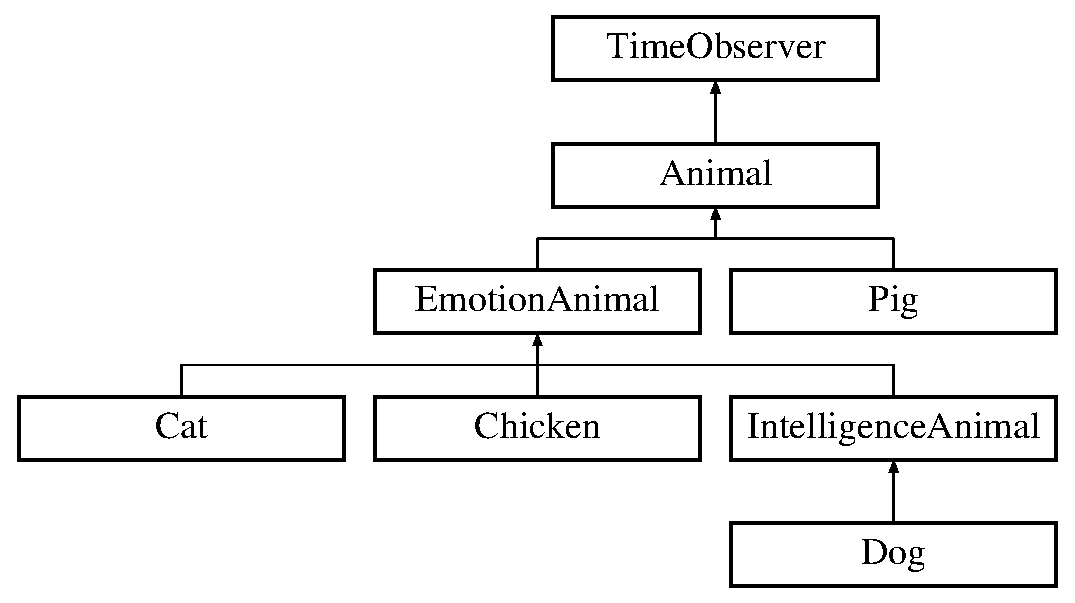
\includegraphics[height=5.000000cm]{class_animal}
\end{center}
\end{figure}
\subsection*{Public Member Functions}
\begin{DoxyCompactItemize}
\item 
\mbox{\Hypertarget{class_animal_acd010252e10da84a05efd43d9bf69279}\label{class_animal_acd010252e10da84a05efd43d9bf69279}} 
string {\bfseries get\+Name} ()
\item 
\mbox{\Hypertarget{class_animal_aa26d5b8f6912f03da2cc64ff0b888972}\label{class_animal_aa26d5b8f6912f03da2cc64ff0b888972}} 
void {\bfseries set\+Name} (string n)
\item 
\mbox{\Hypertarget{class_animal_abd2ffd89b5ad2126ac2af7d31ca6d446}\label{class_animal_abd2ffd89b5ad2126ac2af7d31ca6d446}} 
string {\bfseries get\+Type} ()
\item 
\mbox{\Hypertarget{class_animal_a4b3acac24e7995363c4f130887c3b3ab}\label{class_animal_a4b3acac24e7995363c4f130887c3b3ab}} 
int {\bfseries get\+Age} ()
\item 
\mbox{\Hypertarget{class_animal_a91a574efed96581f15ce99c62dba3778}\label{class_animal_a91a574efed96581f15ce99c62dba3778}} 
void {\bfseries set\+Age} (int a)
\item 
\mbox{\Hypertarget{class_animal_a722be3bcb2f66289160b6932111caf32}\label{class_animal_a722be3bcb2f66289160b6932111caf32}} 
float {\bfseries get\+Weight} ()
\item 
\mbox{\Hypertarget{class_animal_a79b8aaf14511a9624d35fb9e83959270}\label{class_animal_a79b8aaf14511a9624d35fb9e83959270}} 
void {\bfseries set\+Weight} (float w)
\item 
\mbox{\Hypertarget{class_animal_ad5cee2c9d8bdfc27e3eea866f7ed6eea}\label{class_animal_ad5cee2c9d8bdfc27e3eea866f7ed6eea}} 
int {\bfseries get\+Price\+Sell} ()
\item 
\mbox{\Hypertarget{class_animal_aee99154e40d8d538308f803a24bd8314}\label{class_animal_aee99154e40d8d538308f803a24bd8314}} 
virtual void {\bfseries set\+Price\+Sell} (int p)
\item 
\mbox{\Hypertarget{class_animal_a0d329a7e10c3ab3af2f4e9048326c1e2}\label{class_animal_a0d329a7e10c3ab3af2f4e9048326c1e2}} 
int {\bfseries get\+Price\+Buy} ()
\item 
\mbox{\Hypertarget{class_animal_a6ad26fc54e55d2a577bdb0673f9c6c7e}\label{class_animal_a6ad26fc54e55d2a577bdb0673f9c6c7e}} 
virtual void {\bfseries set\+Price\+Buy} (int p)
\item 
\mbox{\Hypertarget{class_animal_a39c25838a7b4dd87e67838cc6e78fae6}\label{class_animal_a39c25838a7b4dd87e67838cc6e78fae6}} 
void {\bfseries sound} ()
\item 
\mbox{\Hypertarget{class_animal_ad018a3798fe7ddf30da60d8f2557701b}\label{class_animal_ad018a3798fe7ddf30da60d8f2557701b}} 
virtual void {\bfseries eat} ()=0
\item 
\mbox{\Hypertarget{class_animal_afcacae4af51b4f3fc88a1354f21dc7a7}\label{class_animal_afcacae4af51b4f3fc88a1354f21dc7a7}} 
virtual void {\bfseries go\+Out} ()=0
\item 
\mbox{\Hypertarget{class_animal_af74e43a1338419fe4582e61e2b4d8d34}\label{class_animal_af74e43a1338419fe4582e61e2b4d8d34}} 
virtual void {\bfseries go\+Back} ()=0
\item 
\mbox{\Hypertarget{class_animal_a6cc3df8555c60352f9c55ca174a9f9df}\label{class_animal_a6cc3df8555c60352f9c55ca174a9f9df}} 
virtual void {\bfseries die} ()=0
\item 
\mbox{\Hypertarget{class_animal_aaa82a4b9ceb712c473d84b87c920043f}\label{class_animal_aaa82a4b9ceb712c473d84b87c920043f}} 
virtual int {\bfseries reproduce} ()=0
\item 
\mbox{\Hypertarget{class_animal_a126acfdd961c2d49373159b256d71b23}\label{class_animal_a126acfdd961c2d49373159b256d71b23}} 
virtual void {\bfseries listen} ()=0
\item 
\mbox{\Hypertarget{class_animal_ae3e210967f50cee3ef1023d985976867}\label{class_animal_ae3e210967f50cee3ef1023d985976867}} 
void {\bfseries add\+Listener} (\hyperlink{class_animal}{Animal} $\ast$a)
\item 
\mbox{\Hypertarget{class_animal_a83e0c4009f62540aca99f0b5ceeb7fdd}\label{class_animal_a83e0c4009f62540aca99f0b5ceeb7fdd}} 
void {\bfseries remove\+Listener} (\hyperlink{class_animal}{Animal} $\ast$a)
\item 
\mbox{\Hypertarget{class_animal_aec682deda01c7165197f7c7eba9ab88c}\label{class_animal_aec682deda01c7165197f7c7eba9ab88c}} 
virtual void {\bfseries on\+Hour\+Change} (int h)=0
\item 
\mbox{\Hypertarget{class_animal_af4b1639570a362dda44948ed483bf94c}\label{class_animal_af4b1639570a362dda44948ed483bf94c}} 
virtual void {\bfseries on\+Day\+Change} (int d)=0
\end{DoxyCompactItemize}
\subsection*{Protected Member Functions}
\begin{DoxyCompactItemize}
\item 
\mbox{\Hypertarget{class_animal_a93ad63b6239f8f18d167034b7948f35a}\label{class_animal_a93ad63b6239f8f18d167034b7948f35a}} 
virtual void {\bfseries print\+Sound} ()=0
\item 
\mbox{\Hypertarget{class_animal_aa1ebce4b14be5e3d38c831b51a7ac307}\label{class_animal_aa1ebce4b14be5e3d38c831b51a7ac307}} 
void {\bfseries notify\+Listener} ()
\end{DoxyCompactItemize}
\subsection*{Protected Attributes}
\begin{DoxyCompactItemize}
\item 
string \hyperlink{class_animal_a9cf3bfd9070daec7b3bbc87cbd958f35}{name}
\item 
\mbox{\Hypertarget{class_animal_a8b120b31083a0561ab9969d5aeb03195}\label{class_animal_a8b120b31083a0561ab9969d5aeb03195}} 
string {\bfseries type}
\item 
\mbox{\Hypertarget{class_animal_a31e4a23bef9596927496de4eb6b9c721}\label{class_animal_a31e4a23bef9596927496de4eb6b9c721}} 
int {\bfseries age}
\item 
\mbox{\Hypertarget{class_animal_a055c4df7dacb89eb4c2ca9bbee11ff24}\label{class_animal_a055c4df7dacb89eb4c2ca9bbee11ff24}} 
float {\bfseries weight}
\item 
\mbox{\Hypertarget{class_animal_ae18bdb6ca2de33354df5d877f159fb5b}\label{class_animal_ae18bdb6ca2de33354df5d877f159fb5b}} 
int {\bfseries price\+Buy}
\item 
\mbox{\Hypertarget{class_animal_a5386cd93699ab24f8faddc3a2bfeea99}\label{class_animal_a5386cd93699ab24f8faddc3a2bfeea99}} 
int {\bfseries price\+Sell}
\item 
\mbox{\Hypertarget{class_animal_a386cf61e5b26f85531a56cdefbae3784}\label{class_animal_a386cf61e5b26f85531a56cdefbae3784}} 
int {\bfseries sound\+Count}
\item 
\mbox{\Hypertarget{class_animal_a4819eec8f0cb2e20cd40328db1d313d8}\label{class_animal_a4819eec8f0cb2e20cd40328db1d313d8}} 
int {\bfseries eat\+Count}
\item 
\mbox{\Hypertarget{class_animal_a15e2ae06f4ce89a2c1a20fa3f919586c}\label{class_animal_a15e2ae06f4ce89a2c1a20fa3f919586c}} 
vector$<$ \hyperlink{class_animal}{Animal} $\ast$ $>$ {\bfseries listeners}
\end{DoxyCompactItemize}


\subsection{Member Data Documentation}
\mbox{\Hypertarget{class_animal_a9cf3bfd9070daec7b3bbc87cbd958f35}\label{class_animal_a9cf3bfd9070daec7b3bbc87cbd958f35}} 
\index{Animal@{Animal}!name@{name}}
\index{name@{name}!Animal@{Animal}}
\subsubsection{\texorpdfstring{name}{name}}
{\footnotesize\ttfamily string Animal\+::name\hspace{0.3cm}{\ttfamily [protected]}}

ten con vat... 

The documentation for this class was generated from the following files\+:\begin{DoxyCompactItemize}
\item 
Animal.\+h\item 
Animal.\+cpp\end{DoxyCompactItemize}

\hypertarget{class_animal_factory}{}\section{Animal\+Factory Class Reference}
\label{class_animal_factory}\index{Animal\+Factory@{Animal\+Factory}}
\subsection*{Public Member Functions}
\begin{DoxyCompactItemize}
\item 
\mbox{\Hypertarget{class_animal_factory_a1f6082d5df78aa84dd5a01404ea27f85}\label{class_animal_factory_a1f6082d5df78aa84dd5a01404ea27f85}} 
\hyperlink{class_animal}{Animal} $\ast$ {\bfseries create\+Animal} (string type)
\end{DoxyCompactItemize}


The documentation for this class was generated from the following files\+:\begin{DoxyCompactItemize}
\item 
Animal\+Factory.\+h\item 
Animal\+Factory.\+cpp\end{DoxyCompactItemize}

\hypertarget{class_animal_manager}{}\section{Animal\+Manager Class Reference}
\label{class_animal_manager}\index{Animal\+Manager@{Animal\+Manager}}
\subsection*{Public Member Functions}
\begin{DoxyCompactItemize}
\item 
\mbox{\Hypertarget{class_animal_manager_a0c047e132bf297a8ecbe153783c7928f}\label{class_animal_manager_a0c047e132bf297a8ecbe153783c7928f}} 
void {\bfseries buy\+Animal} (string type, string name)
\item 
\mbox{\Hypertarget{class_animal_manager_a0706166b7609abae09369aedd309453e}\label{class_animal_manager_a0706166b7609abae09369aedd309453e}} 
void {\bfseries sell\+Animal} (string type, string name)
\item 
\mbox{\Hypertarget{class_animal_manager_ae81755971c331f3539a6bfd83e8f5d33}\label{class_animal_manager_ae81755971c331f3539a6bfd83e8f5d33}} 
void {\bfseries sell\+Animal} (string type)
\item 
\mbox{\Hypertarget{class_animal_manager_a66ed845ca84b2044d20b6061f5e856c8}\label{class_animal_manager_a66ed845ca84b2044d20b6061f5e856c8}} 
void {\bfseries feed\+Animals} ()
\item 
\mbox{\Hypertarget{class_animal_manager_a9d02ca95ac0cc06ce7f442f1e09d20f3}\label{class_animal_manager_a9d02ca95ac0cc06ce7f442f1e09d20f3}} 
void {\bfseries feed\+Animal\+By\+Type} (string type)
\item 
\mbox{\Hypertarget{class_animal_manager_a6f5d8ff7e9032aefc52240c888dcc007}\label{class_animal_manager_a6f5d8ff7e9032aefc52240c888dcc007}} 
void {\bfseries feed\+Animal\+By\+Name} (string name)
\item 
\mbox{\Hypertarget{class_animal_manager_abc80d5035e94b824a4e331f64650601c}\label{class_animal_manager_abc80d5035e94b824a4e331f64650601c}} 
void {\bfseries set\+Resource\+Listener} (\hyperlink{class_resuorce_manager}{Resuorce\+Manager} $\ast$resource)
\end{DoxyCompactItemize}
\subsection*{Protected Attributes}
\begin{DoxyCompactItemize}
\item 
\mbox{\Hypertarget{class_animal_manager_a0f14e3b8559ae93d1dccdc311e8be1c8}\label{class_animal_manager_a0f14e3b8559ae93d1dccdc311e8be1c8}} 
\hyperlink{class_resuorce_manager}{Resuorce\+Manager} $\ast$ {\bfseries resource\+Listener}
\item 
\mbox{\Hypertarget{class_animal_manager_aa3faf53beeaa36ec92fc895b6a6311d4}\label{class_animal_manager_aa3faf53beeaa36ec92fc895b6a6311d4}} 
list$<$ \hyperlink{class_animal}{Animal} $\ast$ $>$ {\bfseries animals}
\end{DoxyCompactItemize}
\subsection*{Friends}
\begin{DoxyCompactItemize}
\item 
\mbox{\Hypertarget{class_animal_manager_aec1739a2a9aeb553d1408cb0b93c096d}\label{class_animal_manager_aec1739a2a9aeb553d1408cb0b93c096d}} 
ostream \& {\bfseries operator$<$$<$} (ostream \&os, \hyperlink{class_animal_manager}{Animal\+Manager} \&am)
\end{DoxyCompactItemize}


The documentation for this class was generated from the following files\+:\begin{DoxyCompactItemize}
\item 
Animal\+Manager.\+h\item 
Animal\+Manager.\+cpp\end{DoxyCompactItemize}

\hypertarget{class_cat}{}\section{Cat Class Reference}
\label{class_cat}\index{Cat@{Cat}}
Inheritance diagram for Cat\+:\begin{figure}[H]
\begin{center}
\leavevmode
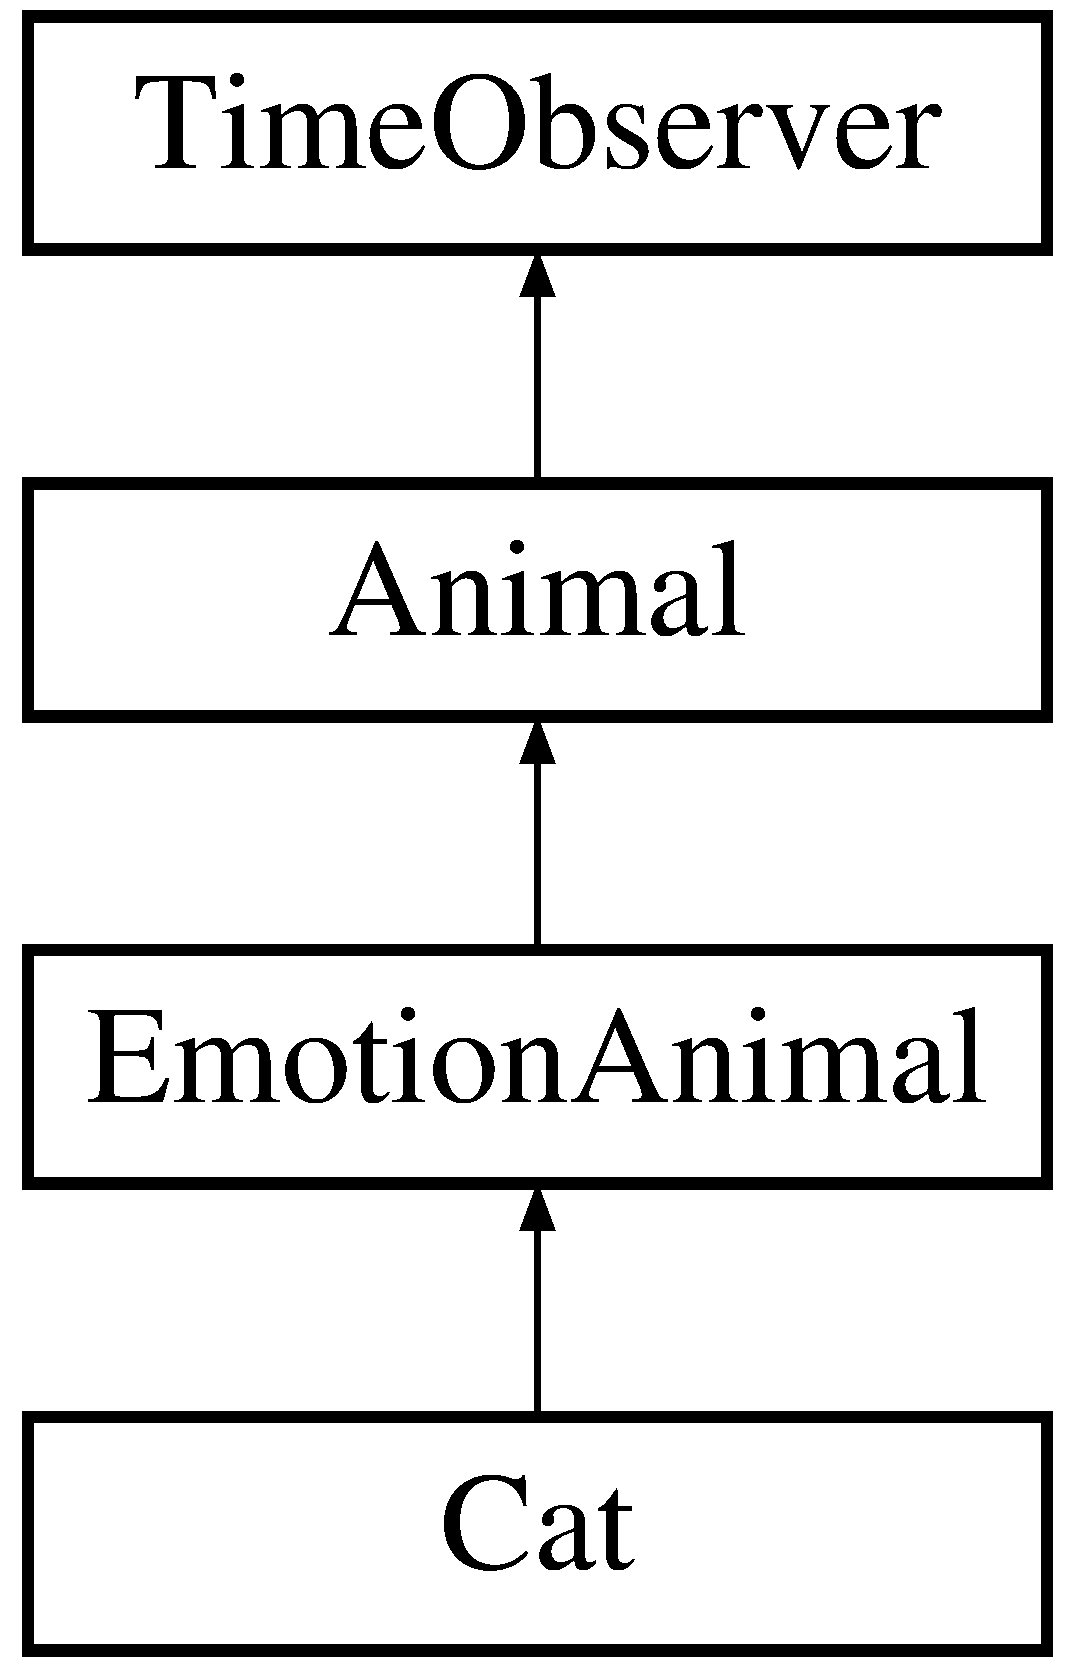
\includegraphics[height=4.000000cm]{class_cat}
\end{center}
\end{figure}
\subsection*{Public Member Functions}
\begin{DoxyCompactItemize}
\item 
\mbox{\Hypertarget{class_cat_a66ece6598afa3205ff6291323ff24964}\label{class_cat_a66ece6598afa3205ff6291323ff24964}} 
virtual void {\bfseries eat} ()
\item 
\mbox{\Hypertarget{class_cat_a6cf8b6c4daf93d9e89cb5665b8df3937}\label{class_cat_a6cf8b6c4daf93d9e89cb5665b8df3937}} 
virtual void {\bfseries go\+Out} ()
\item 
\mbox{\Hypertarget{class_cat_af75e2455e9f7f664d1f5dfd1ece285e7}\label{class_cat_af75e2455e9f7f664d1f5dfd1ece285e7}} 
virtual void {\bfseries go\+Back} ()
\item 
\mbox{\Hypertarget{class_cat_aed1c7db476cda98bddd8f649cb0a4fbf}\label{class_cat_aed1c7db476cda98bddd8f649cb0a4fbf}} 
virtual void {\bfseries die} ()
\item 
\mbox{\Hypertarget{class_cat_ae391b6b7c157fc4f64ed76ea1f4d1b89}\label{class_cat_ae391b6b7c157fc4f64ed76ea1f4d1b89}} 
virtual int {\bfseries reproduce} ()
\item 
\mbox{\Hypertarget{class_cat_aede6b89d75f9a11fc4992a1023bc69c8}\label{class_cat_aede6b89d75f9a11fc4992a1023bc69c8}} 
virtual void {\bfseries listen} ()
\item 
\mbox{\Hypertarget{class_cat_a1776cfe2d85ec783cc2f73a9adb7c09c}\label{class_cat_a1776cfe2d85ec783cc2f73a9adb7c09c}} 
virtual void {\bfseries on\+Hour\+Change} (int h)
\item 
\mbox{\Hypertarget{class_cat_a352d9f1603003aa4bb5e5cd8607cd27a}\label{class_cat_a352d9f1603003aa4bb5e5cd8607cd27a}} 
virtual void {\bfseries on\+Day\+Change} (int d)
\end{DoxyCompactItemize}
\subsection*{Protected Member Functions}
\begin{DoxyCompactItemize}
\item 
\mbox{\Hypertarget{class_cat_a47b3ccbb7f4d63f70ce0c45c3352d19a}\label{class_cat_a47b3ccbb7f4d63f70ce0c45c3352d19a}} 
virtual void {\bfseries print\+Sound} ()
\end{DoxyCompactItemize}
\subsection*{Additional Inherited Members}


The documentation for this class was generated from the following files\+:\begin{DoxyCompactItemize}
\item 
Cat.\+h\item 
Cat.\+cpp\end{DoxyCompactItemize}

\hypertarget{class_chicken}{}\section{Chicken Class Reference}
\label{class_chicken}\index{Chicken@{Chicken}}
Inheritance diagram for Chicken\+:\begin{figure}[H]
\begin{center}
\leavevmode
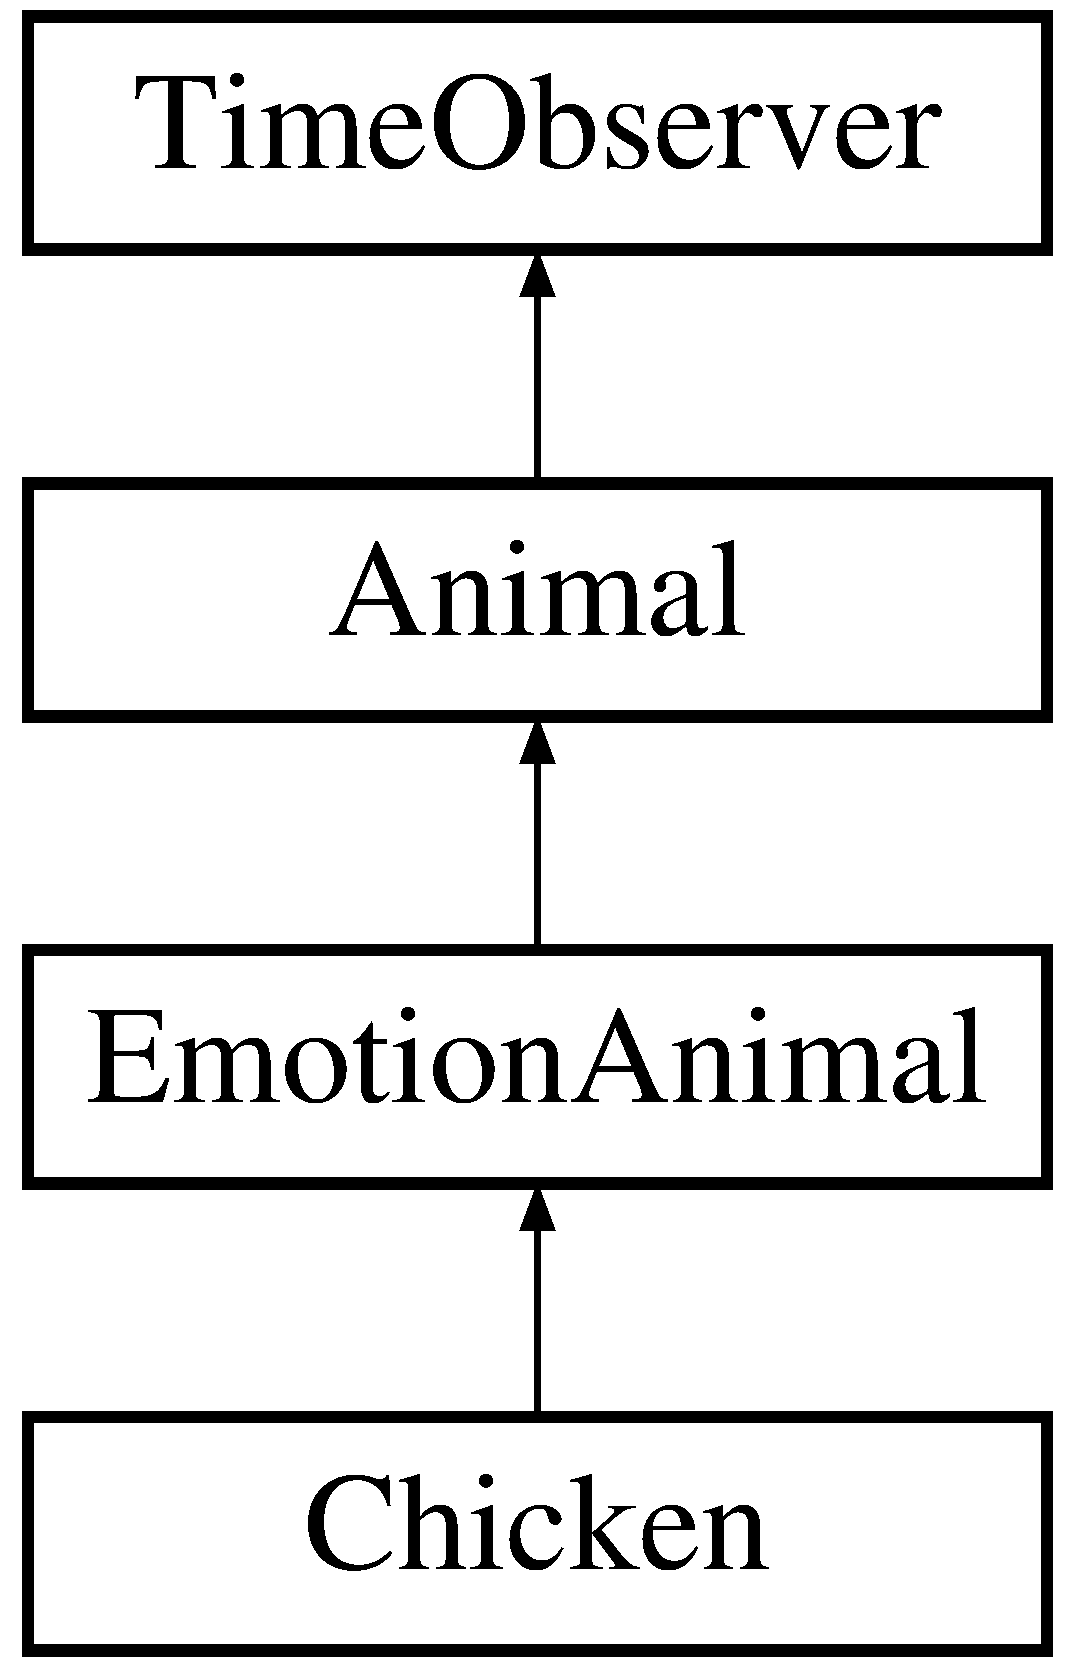
\includegraphics[height=4.000000cm]{class_chicken}
\end{center}
\end{figure}
\subsection*{Public Member Functions}
\begin{DoxyCompactItemize}
\item 
\mbox{\Hypertarget{class_chicken_aa97cec0b7d3f0e781b201b6e266334f2}\label{class_chicken_aa97cec0b7d3f0e781b201b6e266334f2}} 
virtual void {\bfseries eat} ()
\item 
\mbox{\Hypertarget{class_chicken_a327d90f77808e083af04dd9c0f7546f2}\label{class_chicken_a327d90f77808e083af04dd9c0f7546f2}} 
virtual void {\bfseries go\+Out} ()
\item 
\mbox{\Hypertarget{class_chicken_a7c8af6c0cb050c3d0ce2ce9809ead79d}\label{class_chicken_a7c8af6c0cb050c3d0ce2ce9809ead79d}} 
virtual void {\bfseries go\+Back} ()
\item 
\mbox{\Hypertarget{class_chicken_a30db8f1a04f6aa3a4996664e81698f61}\label{class_chicken_a30db8f1a04f6aa3a4996664e81698f61}} 
virtual void {\bfseries die} ()
\item 
\mbox{\Hypertarget{class_chicken_ac967d103a38f616fe48743b7c1fa5118}\label{class_chicken_ac967d103a38f616fe48743b7c1fa5118}} 
virtual int {\bfseries reproduce} ()
\item 
\mbox{\Hypertarget{class_chicken_ab27dad98951f0189fc8e83ca517667c4}\label{class_chicken_ab27dad98951f0189fc8e83ca517667c4}} 
virtual void {\bfseries on\+Hour\+Change} (int h)
\item 
\mbox{\Hypertarget{class_chicken_abd9246cbceeba80e73010e421694d3a4}\label{class_chicken_abd9246cbceeba80e73010e421694d3a4}} 
virtual void {\bfseries on\+Day\+Change} (int d)
\item 
\mbox{\Hypertarget{class_chicken_ab9fccf0929444a4b96baf20fc783a979}\label{class_chicken_ab9fccf0929444a4b96baf20fc783a979}} 
virtual void {\bfseries listen} ()
\end{DoxyCompactItemize}
\subsection*{Protected Member Functions}
\begin{DoxyCompactItemize}
\item 
\mbox{\Hypertarget{class_chicken_a43a91e7cc5bf7958a5052f894f1bfede}\label{class_chicken_a43a91e7cc5bf7958a5052f894f1bfede}} 
virtual void {\bfseries print\+Sound} ()
\end{DoxyCompactItemize}
\subsection*{Additional Inherited Members}


The documentation for this class was generated from the following files\+:\begin{DoxyCompactItemize}
\item 
Chicken.\+h\item 
Chicken.\+cpp\end{DoxyCompactItemize}

\hypertarget{class_dog}{}\section{Dog Class Reference}
\label{class_dog}\index{Dog@{Dog}}
Inheritance diagram for Dog\+:\begin{figure}[H]
\begin{center}
\leavevmode
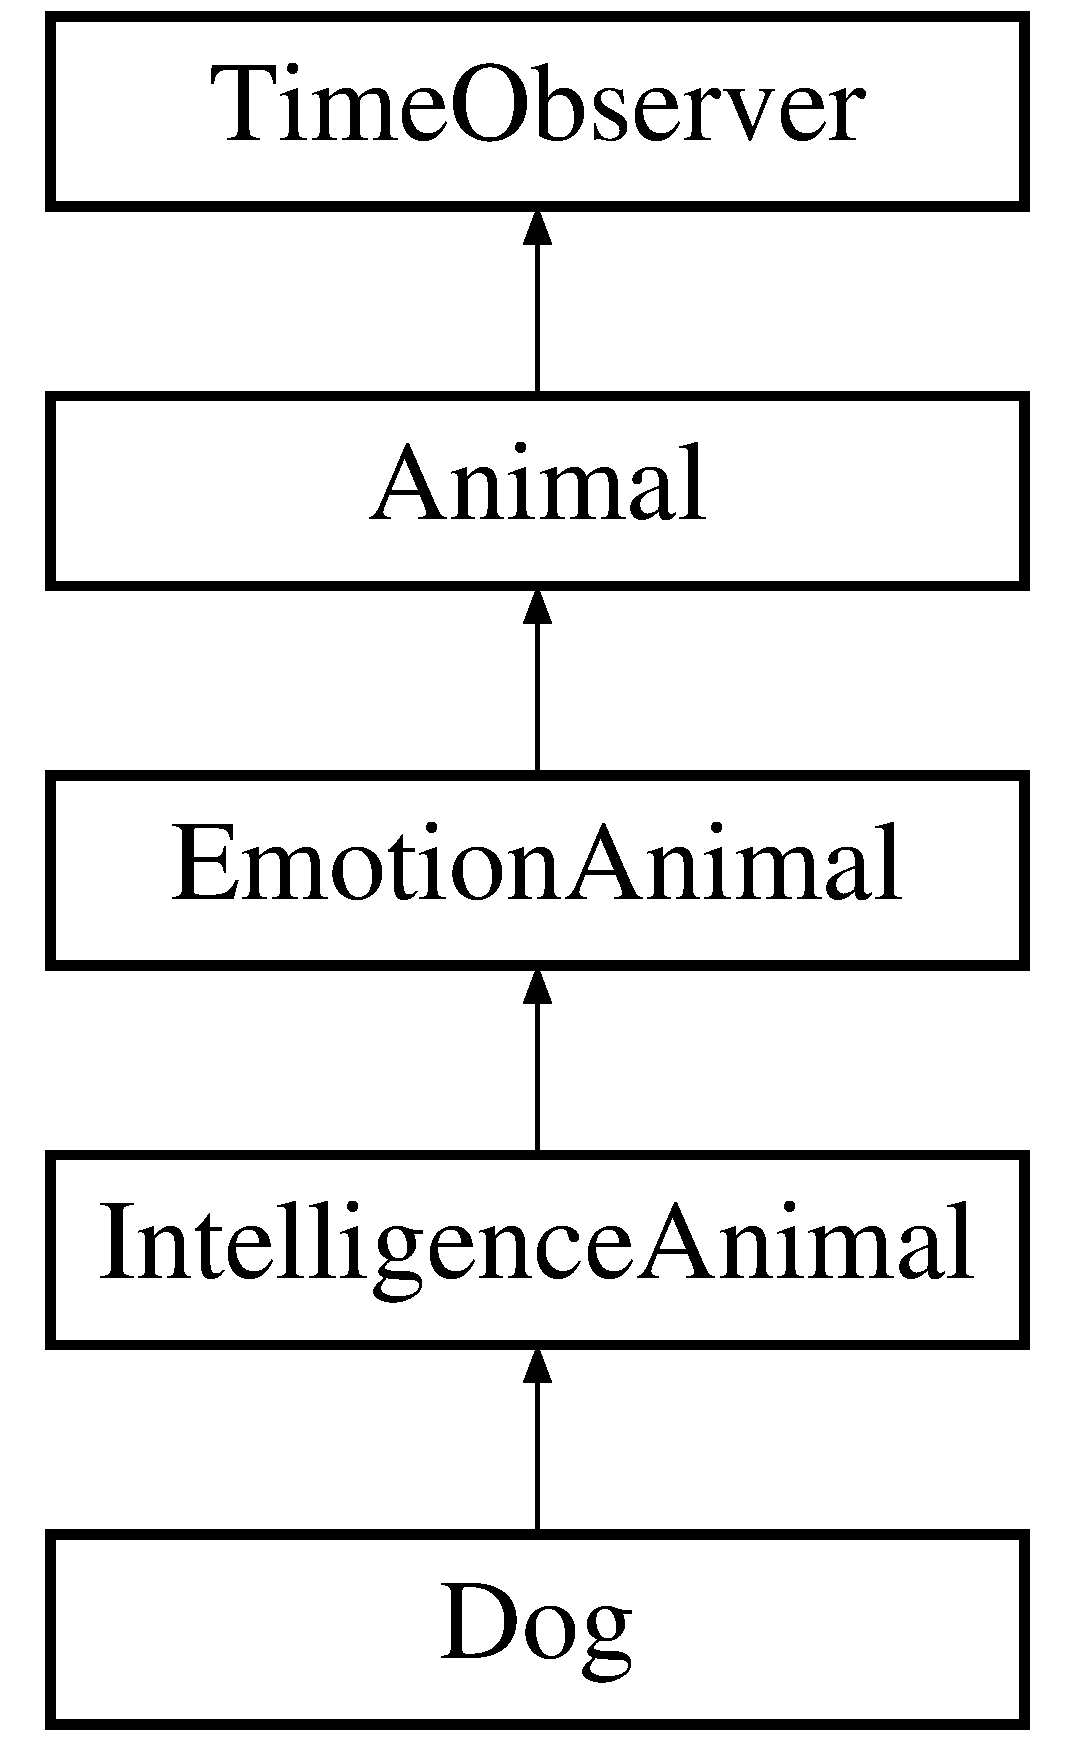
\includegraphics[height=5.000000cm]{class_dog}
\end{center}
\end{figure}
\subsection*{Public Member Functions}
\begin{DoxyCompactItemize}
\item 
\mbox{\Hypertarget{class_dog_aa3ac6ad4799963f3084b347cba19594e}\label{class_dog_aa3ac6ad4799963f3084b347cba19594e}} 
virtual void {\bfseries train} ()
\item 
\mbox{\Hypertarget{class_dog_a03adeca9cd440ef988f9a07a41cc2f18}\label{class_dog_a03adeca9cd440ef988f9a07a41cc2f18}} 
virtual void {\bfseries eat} ()
\item 
\mbox{\Hypertarget{class_dog_a32bc56294e6514c52d68b3e6ceb90768}\label{class_dog_a32bc56294e6514c52d68b3e6ceb90768}} 
virtual void {\bfseries go\+Out} ()
\item 
\mbox{\Hypertarget{class_dog_a41d697efa2242f02bd9a21605407f658}\label{class_dog_a41d697efa2242f02bd9a21605407f658}} 
virtual void {\bfseries go\+Back} ()
\item 
\mbox{\Hypertarget{class_dog_a2d87cfdfd256fe56b0b83249dc11bdae}\label{class_dog_a2d87cfdfd256fe56b0b83249dc11bdae}} 
virtual void {\bfseries die} ()
\item 
\mbox{\Hypertarget{class_dog_a3b8fdd98742fea3b9e438538126edf6d}\label{class_dog_a3b8fdd98742fea3b9e438538126edf6d}} 
virtual int {\bfseries reproduce} ()
\item 
\mbox{\Hypertarget{class_dog_a6becf925701be98c59817d2a6697129c}\label{class_dog_a6becf925701be98c59817d2a6697129c}} 
virtual void {\bfseries listen} ()
\item 
\mbox{\Hypertarget{class_dog_a4820ede4339708ac557d05f70518e08b}\label{class_dog_a4820ede4339708ac557d05f70518e08b}} 
virtual void {\bfseries on\+Hour\+Change} (int h)
\item 
\mbox{\Hypertarget{class_dog_a03fdea43325495ca60f1aad753b0fc6a}\label{class_dog_a03fdea43325495ca60f1aad753b0fc6a}} 
virtual void {\bfseries on\+Day\+Change} (int d)
\end{DoxyCompactItemize}
\subsection*{Protected Member Functions}
\begin{DoxyCompactItemize}
\item 
\mbox{\Hypertarget{class_dog_a042e0f6390025ea229fdba51a60c2ca7}\label{class_dog_a042e0f6390025ea229fdba51a60c2ca7}} 
virtual void {\bfseries print\+Sound} ()
\end{DoxyCompactItemize}
\subsection*{Additional Inherited Members}


The documentation for this class was generated from the following files\+:\begin{DoxyCompactItemize}
\item 
Dog.\+h\item 
Dog.\+cpp\end{DoxyCompactItemize}

\hypertarget{class_emotion_animal}{}\section{Emotion\+Animal Class Reference}
\label{class_emotion_animal}\index{Emotion\+Animal@{Emotion\+Animal}}
Inheritance diagram for Emotion\+Animal\+:\begin{figure}[H]
\begin{center}
\leavevmode
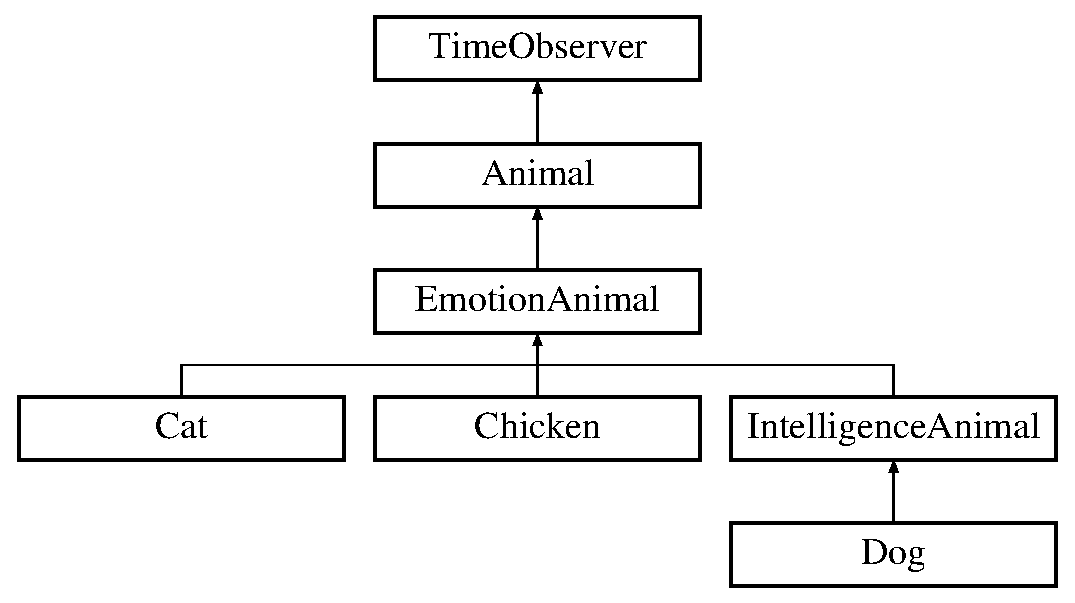
\includegraphics[height=5.000000cm]{class_emotion_animal}
\end{center}
\end{figure}
\subsection*{Public Member Functions}
\begin{DoxyCompactItemize}
\item 
\mbox{\Hypertarget{class_emotion_animal_ae075ddea4c14459fc47dd8fb6b986676}\label{class_emotion_animal_ae075ddea4c14459fc47dd8fb6b986676}} 
int {\bfseries get\+Happy\+Index} ()
\item 
\mbox{\Hypertarget{class_emotion_animal_af269fd4dc612625c77ce55667502a092}\label{class_emotion_animal_af269fd4dc612625c77ce55667502a092}} 
void {\bfseries set\+Happy\+Index} (int i)
\item 
\mbox{\Hypertarget{class_emotion_animal_ad112df6f803ac02b701558c4765c8dc9}\label{class_emotion_animal_ad112df6f803ac02b701558c4765c8dc9}} 
virtual void {\bfseries eat} ()=0
\item 
\mbox{\Hypertarget{class_emotion_animal_a4961194875c3c286808f2aa2a23eec3d}\label{class_emotion_animal_a4961194875c3c286808f2aa2a23eec3d}} 
virtual void {\bfseries go\+Out} ()=0
\item 
\mbox{\Hypertarget{class_emotion_animal_aee6f0e1c1bf618172d59a79fe1630190}\label{class_emotion_animal_aee6f0e1c1bf618172d59a79fe1630190}} 
virtual void {\bfseries go\+Back} ()=0
\item 
\mbox{\Hypertarget{class_emotion_animal_ad89a20ca48b79c9fc5681d6b5a811330}\label{class_emotion_animal_ad89a20ca48b79c9fc5681d6b5a811330}} 
virtual void {\bfseries die} ()=0
\item 
\mbox{\Hypertarget{class_emotion_animal_a499ff4778d256bac4cc3604ff764e371}\label{class_emotion_animal_a499ff4778d256bac4cc3604ff764e371}} 
virtual int {\bfseries reproduce} ()=0
\item 
\mbox{\Hypertarget{class_emotion_animal_a9740606110f30a35c2a64fda0200ea6f}\label{class_emotion_animal_a9740606110f30a35c2a64fda0200ea6f}} 
virtual void {\bfseries listen} ()=0
\item 
\mbox{\Hypertarget{class_emotion_animal_a28e538a0afde42d04fc68c3da53bffbf}\label{class_emotion_animal_a28e538a0afde42d04fc68c3da53bffbf}} 
virtual void {\bfseries on\+Hour\+Change} (int h)=0
\item 
\mbox{\Hypertarget{class_emotion_animal_a4c065f7aa86b04e35a5caf5c5753ae42}\label{class_emotion_animal_a4c065f7aa86b04e35a5caf5c5753ae42}} 
virtual void {\bfseries on\+Day\+Change} (int d)=0
\end{DoxyCompactItemize}
\subsection*{Protected Member Functions}
\begin{DoxyCompactItemize}
\item 
\mbox{\Hypertarget{class_emotion_animal_acfa023a678c278d8da78adac0bc3234f}\label{class_emotion_animal_acfa023a678c278d8da78adac0bc3234f}} 
virtual void {\bfseries print\+Sound} ()=0
\end{DoxyCompactItemize}
\subsection*{Protected Attributes}
\begin{DoxyCompactItemize}
\item 
\mbox{\Hypertarget{class_emotion_animal_a6619eb4ba696ac2892851cb3dacd863d}\label{class_emotion_animal_a6619eb4ba696ac2892851cb3dacd863d}} 
int {\bfseries happy\+Index}
\end{DoxyCompactItemize}


The documentation for this class was generated from the following files\+:\begin{DoxyCompactItemize}
\item 
Emotion\+Animal.\+h\item 
Emotion\+Animal.\+cpp\end{DoxyCompactItemize}

\hypertarget{class_intelligence_animal}{}\section{Intelligence\+Animal Class Reference}
\label{class_intelligence_animal}\index{Intelligence\+Animal@{Intelligence\+Animal}}
Inheritance diagram for Intelligence\+Animal\+:\begin{figure}[H]
\begin{center}
\leavevmode
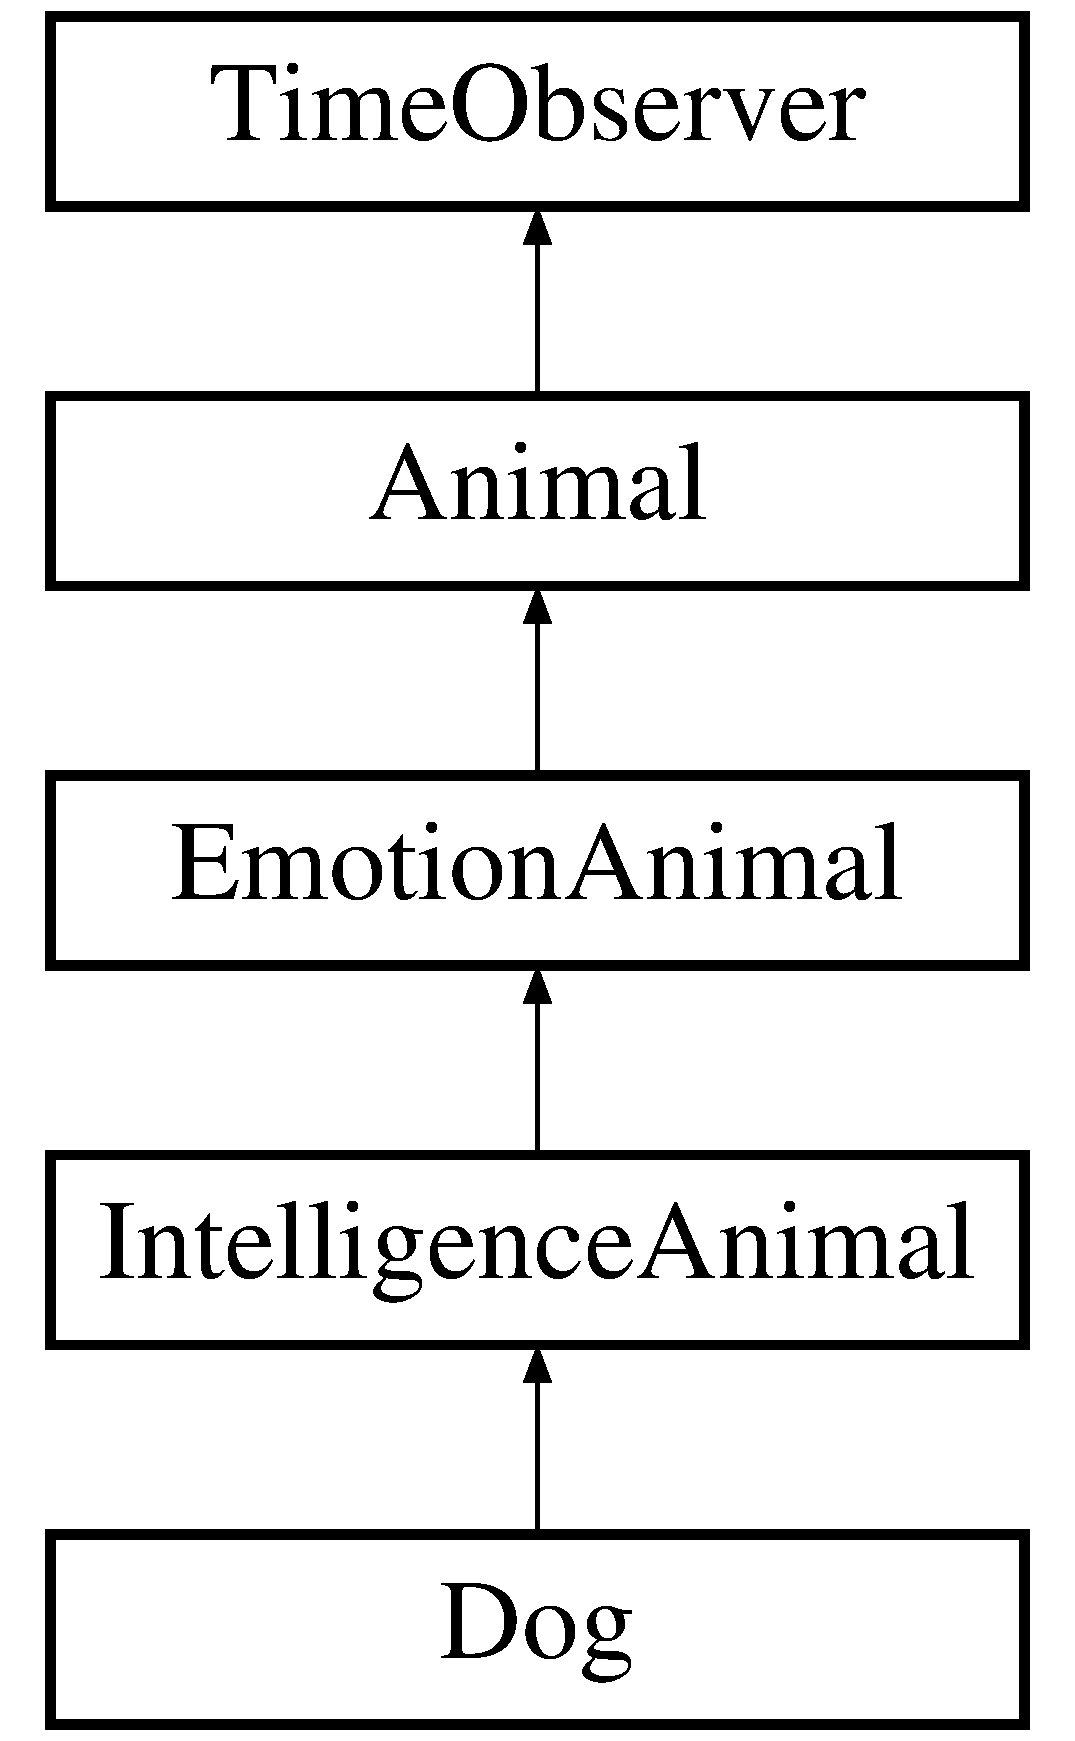
\includegraphics[height=5.000000cm]{class_intelligence_animal}
\end{center}
\end{figure}
\subsection*{Public Member Functions}
\begin{DoxyCompactItemize}
\item 
\mbox{\Hypertarget{class_intelligence_animal_a3d1742ff1c76aed9394748f11d5d8789}\label{class_intelligence_animal_a3d1742ff1c76aed9394748f11d5d8789}} 
virtual void {\bfseries train} ()=0
\item 
\mbox{\Hypertarget{class_intelligence_animal_aeb924c39e9496e3775b0ef2af35c638f}\label{class_intelligence_animal_aeb924c39e9496e3775b0ef2af35c638f}} 
virtual void {\bfseries eat} ()=0
\item 
\mbox{\Hypertarget{class_intelligence_animal_af58201f17c0847f0a92154462d1fa627}\label{class_intelligence_animal_af58201f17c0847f0a92154462d1fa627}} 
virtual void {\bfseries go\+Out} ()=0
\item 
\mbox{\Hypertarget{class_intelligence_animal_aa09abbbe91dddc5e37a01d17bc5423e2}\label{class_intelligence_animal_aa09abbbe91dddc5e37a01d17bc5423e2}} 
virtual void {\bfseries go\+Back} ()=0
\item 
\mbox{\Hypertarget{class_intelligence_animal_ada72ecbbe6cfcbdf7be0000915f0b69e}\label{class_intelligence_animal_ada72ecbbe6cfcbdf7be0000915f0b69e}} 
virtual void {\bfseries die} ()=0
\item 
\mbox{\Hypertarget{class_intelligence_animal_ab8374471442da78816c4f082a907b881}\label{class_intelligence_animal_ab8374471442da78816c4f082a907b881}} 
virtual int {\bfseries reproduce} ()=0
\item 
\mbox{\Hypertarget{class_intelligence_animal_aeb33e78d2fa3b5f2e5ef84f5baf916f7}\label{class_intelligence_animal_aeb33e78d2fa3b5f2e5ef84f5baf916f7}} 
virtual void {\bfseries listen} ()=0
\item 
\mbox{\Hypertarget{class_intelligence_animal_a9bc1ebd1a95082178b3e83dbeee16415}\label{class_intelligence_animal_a9bc1ebd1a95082178b3e83dbeee16415}} 
virtual void {\bfseries on\+Hour\+Change} (int h)=0
\item 
\mbox{\Hypertarget{class_intelligence_animal_a7a96244e5e54f37649c27513af122983}\label{class_intelligence_animal_a7a96244e5e54f37649c27513af122983}} 
virtual void {\bfseries on\+Day\+Change} (int d)=0
\item 
\mbox{\Hypertarget{class_intelligence_animal_a6d5904db3250bd5b94234705abc5b7bb}\label{class_intelligence_animal_a6d5904db3250bd5b94234705abc5b7bb}} 
virtual int {\bfseries get\+Food\+Unit} ()=0
\end{DoxyCompactItemize}
\subsection*{Protected Member Functions}
\begin{DoxyCompactItemize}
\item 
\mbox{\Hypertarget{class_intelligence_animal_a40e0aae3c7b4c4aa4c7e75891243996b}\label{class_intelligence_animal_a40e0aae3c7b4c4aa4c7e75891243996b}} 
virtual void {\bfseries print\+Sound} ()=0
\end{DoxyCompactItemize}
\subsection*{Protected Attributes}
\begin{DoxyCompactItemize}
\item 
\mbox{\Hypertarget{class_intelligence_animal_a6e3849ba9edcfe0c616feb0abce90bd6}\label{class_intelligence_animal_a6e3849ba9edcfe0c616feb0abce90bd6}} 
int {\bfseries intelligence\+Index}
\end{DoxyCompactItemize}


The documentation for this class was generated from the following files\+:\begin{DoxyCompactItemize}
\item 
Intelligence\+Animal.\+h\item 
Intelligence\+Animal.\+cpp\end{DoxyCompactItemize}

\hypertarget{class_mac_donald}{}\section{Mac\+Donald Class Reference}
\label{class_mac_donald}\index{Mac\+Donald@{Mac\+Donald}}
\subsection*{Public Member Functions}
\begin{DoxyCompactItemize}
\item 
\mbox{\Hypertarget{class_mac_donald_af1307eccf048a825243c17c1be3ed178}\label{class_mac_donald_af1307eccf048a825243c17c1be3ed178}} 
void {\bfseries Menu} ()
\item 
\mbox{\Hypertarget{class_mac_donald_a9c0f7d6ff84ae4200791722d27546596}\label{class_mac_donald_a9c0f7d6ff84ae4200791722d27546596}} 
int {\bfseries Select\+Action} ()
\item 
\mbox{\Hypertarget{class_mac_donald_aa3658fd709164100735bdb280d72b9a0}\label{class_mac_donald_aa3658fd709164100735bdb280d72b9a0}} 
void {\bfseries Mac\+Donald\+Activities} ()
\item 
\mbox{\Hypertarget{class_mac_donald_a72b66aa4de048466d5cb5efe4a2f2e80}\label{class_mac_donald_a72b66aa4de048466d5cb5efe4a2f2e80}} 
char {\bfseries Inputname} (char)
\end{DoxyCompactItemize}


The documentation for this class was generated from the following files\+:\begin{DoxyCompactItemize}
\item 
Mac\+Donald.\+h\item 
Mac\+Donald.\+cpp\end{DoxyCompactItemize}

\hypertarget{class_pig}{}\section{Pig Class Reference}
\label{class_pig}\index{Pig@{Pig}}
Inheritance diagram for Pig\+:\begin{figure}[H]
\begin{center}
\leavevmode
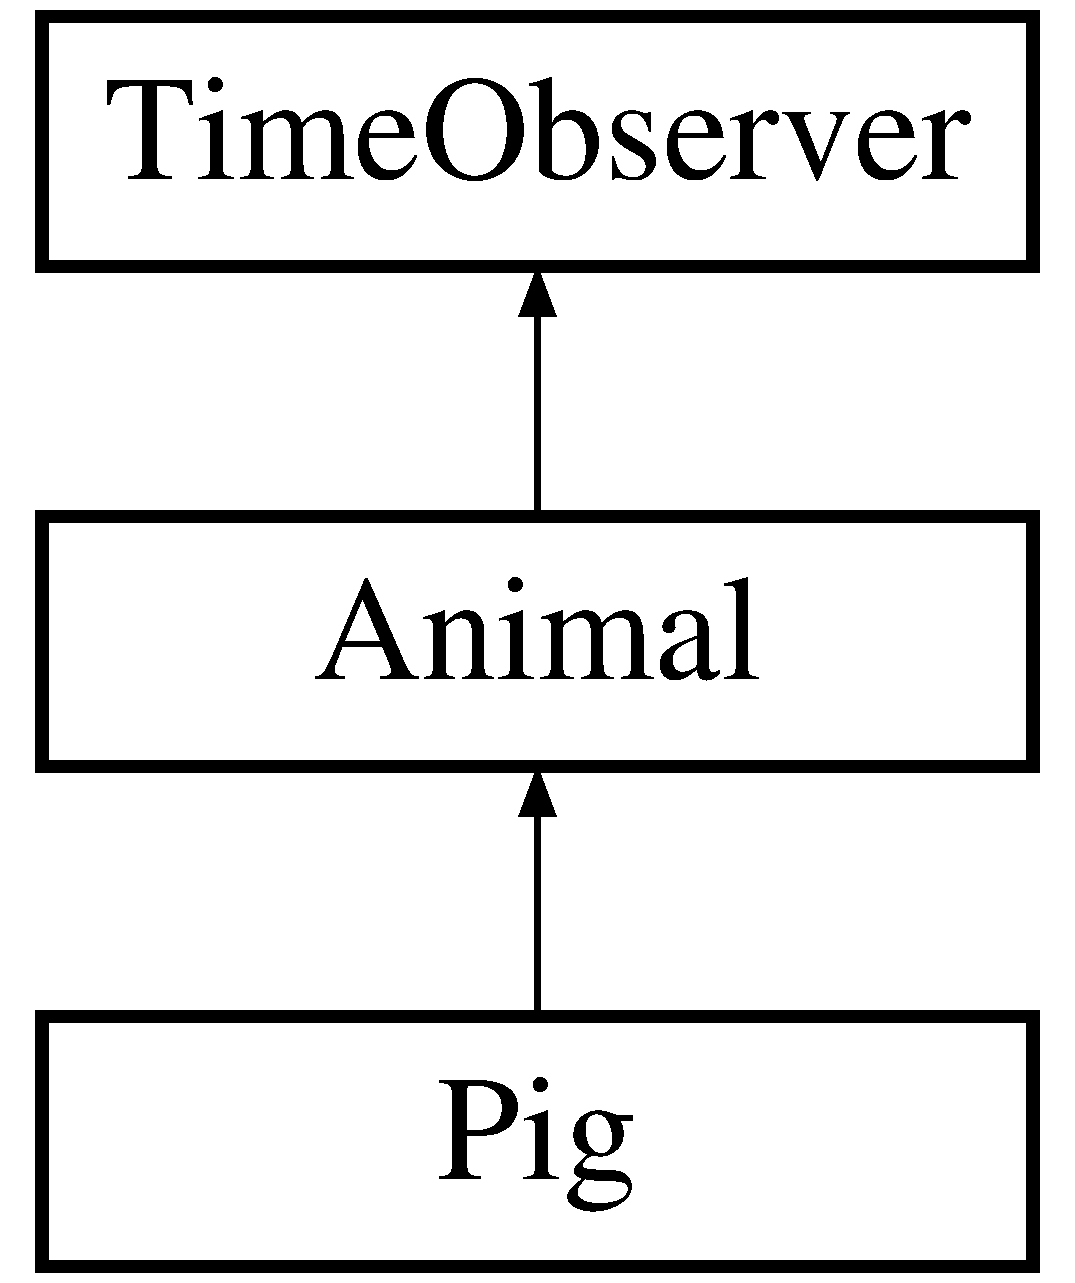
\includegraphics[height=3.000000cm]{class_pig}
\end{center}
\end{figure}
\subsection*{Public Member Functions}
\begin{DoxyCompactItemize}
\item 
\mbox{\Hypertarget{class_pig_a0211e2fe87af7df616125ea0c3c49b9b}\label{class_pig_a0211e2fe87af7df616125ea0c3c49b9b}} 
virtual void {\bfseries set\+Price\+Sell} ()
\item 
\mbox{\Hypertarget{class_pig_a101d2ba5c0384f287a4d762c0b103929}\label{class_pig_a101d2ba5c0384f287a4d762c0b103929}} 
virtual void {\bfseries eat} ()
\item 
\mbox{\Hypertarget{class_pig_a346e5a198e9a2208afda64f271e18ce4}\label{class_pig_a346e5a198e9a2208afda64f271e18ce4}} 
virtual void {\bfseries go\+Out} ()
\item 
\mbox{\Hypertarget{class_pig_a8910acc68ea058501b8bb9d2e104f3db}\label{class_pig_a8910acc68ea058501b8bb9d2e104f3db}} 
virtual void {\bfseries go\+Back} ()
\item 
\mbox{\Hypertarget{class_pig_ac6f4adb5d005de651af8b2769f693638}\label{class_pig_ac6f4adb5d005de651af8b2769f693638}} 
virtual void {\bfseries die} ()
\item 
\mbox{\Hypertarget{class_pig_a50a4bb2ccc915d430270b032a463de66}\label{class_pig_a50a4bb2ccc915d430270b032a463de66}} 
virtual int {\bfseries reproduce} ()
\item 
\mbox{\Hypertarget{class_pig_a378287d4b572a3d803e2066ec1a5176a}\label{class_pig_a378287d4b572a3d803e2066ec1a5176a}} 
virtual void {\bfseries listen} ()
\item 
\mbox{\Hypertarget{class_pig_a23b39de69985c6128a71d6f2f8bf034a}\label{class_pig_a23b39de69985c6128a71d6f2f8bf034a}} 
virtual void {\bfseries on\+Hour\+Change} (int h)
\item 
\mbox{\Hypertarget{class_pig_a217d0b26a1919076b5f0d8b5869ab8cc}\label{class_pig_a217d0b26a1919076b5f0d8b5869ab8cc}} 
virtual void {\bfseries on\+Day\+Change} (int d)
\end{DoxyCompactItemize}
\subsection*{Protected Member Functions}
\begin{DoxyCompactItemize}
\item 
\mbox{\Hypertarget{class_pig_ab16375db4a149025ea7b2332db7dc519}\label{class_pig_ab16375db4a149025ea7b2332db7dc519}} 
virtual void {\bfseries print\+Sound} ()
\end{DoxyCompactItemize}
\subsection*{Additional Inherited Members}


The documentation for this class was generated from the following files\+:\begin{DoxyCompactItemize}
\item 
Pig.\+h\item 
Pig.\+cpp\end{DoxyCompactItemize}

\hypertarget{class_resuorce_manager}{}\section{Resuorce\+Manager Class Reference}
\label{class_resuorce_manager}\index{Resuorce\+Manager@{Resuorce\+Manager}}
\subsection*{Public Member Functions}
\begin{DoxyCompactItemize}
\item 
\mbox{\Hypertarget{class_resuorce_manager_ab695c8e1d5832a7c8584ab76eb5c7e96}\label{class_resuorce_manager_ab695c8e1d5832a7c8584ab76eb5c7e96}} 
bool {\bfseries buy\+Food} (int m)
\item 
\mbox{\Hypertarget{class_resuorce_manager_ac36a816e1164e3199e6f0747d9476e3c}\label{class_resuorce_manager_ac36a816e1164e3199e6f0747d9476e3c}} 
bool {\bfseries on\+Buy\+Animal} (int price)
\item 
\mbox{\Hypertarget{class_resuorce_manager_ab534e16078bff88c9c77a017b4ee87c4}\label{class_resuorce_manager_ab534e16078bff88c9c77a017b4ee87c4}} 
bool {\bfseries on\+Sell\+Animal} (int price)
\item 
\mbox{\Hypertarget{class_resuorce_manager_a2d14b617098ad105ad90fa135128f35f}\label{class_resuorce_manager_a2d14b617098ad105ad90fa135128f35f}} 
bool {\bfseries on\+Feed\+Animal} (int food\+Count)
\end{DoxyCompactItemize}
\subsection*{Protected Attributes}
\begin{DoxyCompactItemize}
\item 
\mbox{\Hypertarget{class_resuorce_manager_ab56d204cee3db3f1c0ecd49b457a6de0}\label{class_resuorce_manager_ab56d204cee3db3f1c0ecd49b457a6de0}} 
int {\bfseries food}
\item 
\mbox{\Hypertarget{class_resuorce_manager_ab305ccf6a9c242ddfd736baeef1f7463}\label{class_resuorce_manager_ab305ccf6a9c242ddfd736baeef1f7463}} 
int {\bfseries money}
\end{DoxyCompactItemize}
\subsection*{Friends}
\begin{DoxyCompactItemize}
\item 
\mbox{\Hypertarget{class_resuorce_manager_aad53dd7ece0ac1d6fd4359b868cf2c6c}\label{class_resuorce_manager_aad53dd7ece0ac1d6fd4359b868cf2c6c}} 
ostream \& {\bfseries operator$<$$<$} (ostream \&os, \hyperlink{class_resuorce_manager}{Resuorce\+Manager} \&r)
\end{DoxyCompactItemize}


The documentation for this class was generated from the following files\+:\begin{DoxyCompactItemize}
\item 
Resuorce\+Manager.\+h\item 
Resuorce\+Manager.\+cpp\end{DoxyCompactItemize}

\hypertarget{class_time_manager}{}\section{Time\+Manager Class Reference}
\label{class_time_manager}\index{Time\+Manager@{Time\+Manager}}
\subsection*{Public Member Functions}
\begin{DoxyCompactItemize}
\item 
\mbox{\Hypertarget{class_time_manager_a0ac1e15f52e5eea41a2d18674cf72715}\label{class_time_manager_a0ac1e15f52e5eea41a2d18674cf72715}} 
int {\bfseries get\+G\+Day} ()
\item 
\mbox{\Hypertarget{class_time_manager_a379a4916e515c90e3370a1da629cde8c}\label{class_time_manager_a379a4916e515c90e3370a1da629cde8c}} 
int {\bfseries get\+G\+Hour} ()
\item 
\mbox{\Hypertarget{class_time_manager_a50b4408595800df3d8849768fa04b1ab}\label{class_time_manager_a50b4408595800df3d8849768fa04b1ab}} 
void {\bfseries covert\+Time} ()
\item 
\mbox{\Hypertarget{class_time_manager_a6f58612f76771bba8b5bd31add3515f4}\label{class_time_manager_a6f58612f76771bba8b5bd31add3515f4}} 
void {\bfseries add\+Time\+Obsever} (\hyperlink{class_time_observer}{Time\+Observer} $\ast$observer)
\end{DoxyCompactItemize}
\subsection*{Static Public Member Functions}
\begin{DoxyCompactItemize}
\item 
\mbox{\Hypertarget{class_time_manager_a5f583a47c375aca352161eaedd24a326}\label{class_time_manager_a5f583a47c375aca352161eaedd24a326}} 
static \hyperlink{class_time_manager}{Time\+Manager} $\ast$ {\bfseries get\+Instance} ()
\end{DoxyCompactItemize}


The documentation for this class was generated from the following files\+:\begin{DoxyCompactItemize}
\item 
Time\+Manager.\+h\item 
Time\+Manager.\+cpp\end{DoxyCompactItemize}

\hypertarget{class_time_observer}{}\section{Time\+Observer Class Reference}
\label{class_time_observer}\index{Time\+Observer@{Time\+Observer}}
Inheritance diagram for Time\+Observer\+:\begin{figure}[H]
\begin{center}
\leavevmode
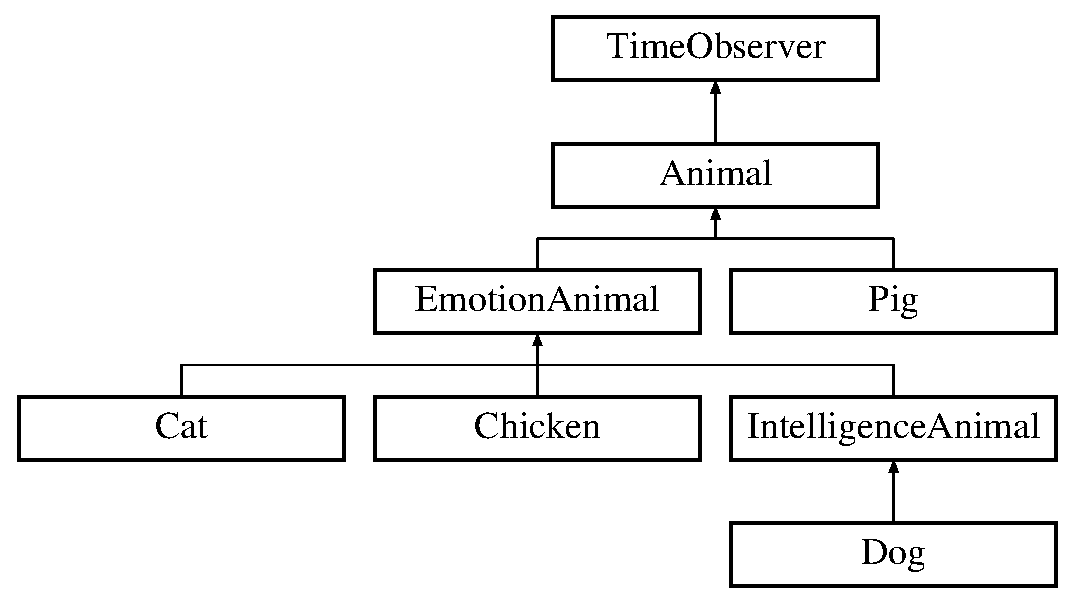
\includegraphics[height=5.000000cm]{class_time_observer}
\end{center}
\end{figure}
\subsection*{Public Member Functions}
\begin{DoxyCompactItemize}
\item 
\mbox{\Hypertarget{class_time_observer_ad544685a6cdd7f7fe75a7696c297cdd7}\label{class_time_observer_ad544685a6cdd7f7fe75a7696c297cdd7}} 
virtual void {\bfseries on\+Day\+Change} (int d)=0
\item 
\mbox{\Hypertarget{class_time_observer_aa9bb5f414aca97a7b06ea4c9f4638171}\label{class_time_observer_aa9bb5f414aca97a7b06ea4c9f4638171}} 
virtual void {\bfseries on\+Hour\+Change} (int h)=0
\end{DoxyCompactItemize}


The documentation for this class was generated from the following files\+:\begin{DoxyCompactItemize}
\item 
Time\+Observer.\+h\item 
Time\+Observer.\+cpp\end{DoxyCompactItemize}

\hypertarget{class_utils}{}\section{Utils Class Reference}
\label{class_utils}\index{Utils@{Utils}}


The documentation for this class was generated from the following files\+:\begin{DoxyCompactItemize}
\item 
Utils.\+h\item 
Utils.\+cpp\end{DoxyCompactItemize}

%--- End generated contents ---

% Index
\backmatter
\newpage
\phantomsection
\clearemptydoublepage
\addcontentsline{toc}{chapter}{Index}
\printindex

\end{document}
